% !TEX program = xelatex
\documentclass[aspectratio=169,12pt]{beamer}

% ── Theme ────────────────────────────────────────────────────────────────────
\usetheme{metropolis}
\usepackage{appendixnumberbeamer}
\usepackage{booktabs}
\usepackage{tikz}
\usetikzlibrary{arrows.meta,positioning,shapes.geometric,fit,calc,decorations.pathreplacing}
\usepackage{fontawesome5}
\usepackage{xcolor}
\usepackage{graphicx}
\usepackage{adjustbox}
\usepackage{array}

% ── Colours ──────────────────────────────────────────────────────────────────
\definecolor{accent}{HTML}{2563EB}    % blue
\definecolor{accent2}{HTML}{059669}   % green
\definecolor{accent3}{HTML}{D97706}   % amber
\definecolor{accent4}{HTML}{DC2626}   % red
\definecolor{amber}{HTML}{F59E0B}     % amber for tikz fills
\definecolor{lightbg}{HTML}{F0F4FF}
\definecolor{darkbg}{HTML}{1E293B}

\setbeamercolor{frametitle}{bg=darkbg, fg=white}
\setbeamercolor{progress bar}{fg=accent}
\setbeamercolor{alerted text}{fg=accent}

% ── Metadata ─────────────────────────────────────────────────────────────────
\title{Agentic AI for Banking}
\subtitle{From Documents to Decisions --- Autonomously}
\author{SFI Masterclass}
\date{2026}
\institute{}

\begin{document}

% ═══════════════════════════════════════════════════════════════════════════════
% TITLE
% ═══════════════════════════════════════════════════════════════════════════════
\begin{frame}[plain]
  \maketitle
\end{frame}

% ═══════════════════════════════════════════════════════════════════════════════
% OUTLINE
% ═══════════════════════════════════════════════════════════════════════════════
\begin{frame}{Roadmap}
  \begin{columns}[T]
    \begin{column}{0.48\textwidth}
      \textbf{\color{accent} Part I --- Concepts}
      \begin{enumerate}
        \item The AI Revolution in 60 Seconds
        \item What LLMs Can (and Can't) Do
        \item RAG: Grounding AI in Facts
        \item Agents: AI That \emph{Acts}
      \end{enumerate}
    \end{column}
    \begin{column}{0.48\textwidth}
      \textbf{\color{accent2} Part II --- Live Demo}
      \begin{enumerate}\setcounter{enumi}{4}
        \item Hands-On: Analysing 10-K Filings
        \item From Prototype to Production
        \item The Banking Opportunity
        \item Risks \& Governance
      \end{enumerate}
    \end{column}
  \end{columns}
\end{frame}

% ═══════════════════════════════════════════════════════════════════════════════
% 1. THE AI REVOLUTION
% ═══════════════════════════════════════════════════════════════════════════════
\section{The AI Revolution}

\begin{frame}{What Changed?}
  \begin{center}
    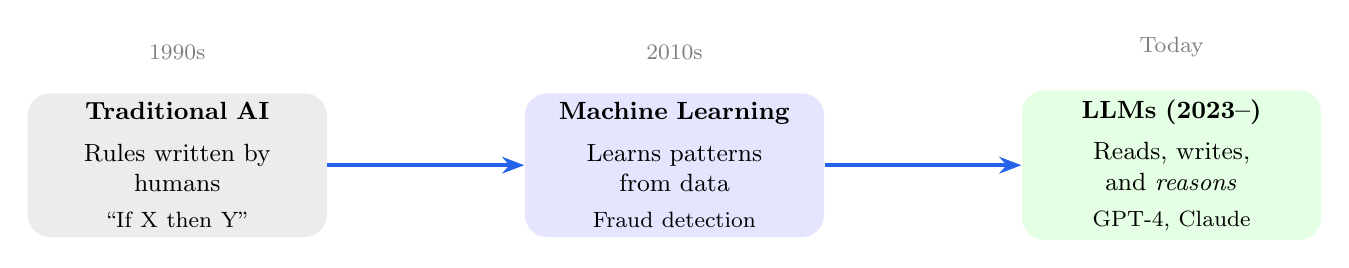
\begin{tikzpicture}[
      box/.style={rounded corners=8pt, minimum width=3.8cm, minimum height=1.8cm,
                  text width=3.4cm, align=center, font=\small},
      arr/.style={-{Stealth[length=8pt]}, line width=1.5pt, accent}
    ]
      \node[box, fill=gray!15] (old) {
        \textbf{Traditional AI}\\[4pt]
        Rules written by\\humans\\[2pt]
        {\footnotesize ``If X then Y''}
      };
      \node[box, fill=blue!10, right=2.5cm of old] (ml) {
        \textbf{Machine Learning}\\[4pt]
        Learns patterns\\from data\\[2pt]
        {\footnotesize Fraud detection}
      };
      \node[box, fill=green!10, right=2.5cm of ml] (llm) {
        \textbf{LLMs (2023--)}\\[4pt]
        Reads, writes,\\and \emph{reasons}\\[2pt]
        {\footnotesize GPT-4, Claude}
      };

      \draw[arr] (old) -- (ml);
      \draw[arr] (ml) -- (llm);

      \node[above=0.3cm of old, font=\footnotesize\color{gray}] {1990s};
      \node[above=0.3cm of ml, font=\footnotesize\color{gray}] {2010s};
      \node[above=0.3cm of llm, font=\footnotesize\color{gray}] {Today};
    \end{tikzpicture}
  \end{center}

  \vspace{0.5cm}
  \begin{alertblock}{The breakthrough}
    For the first time, machines can \textbf{read}, \textbf{understand}, and \textbf{generate}
    human-quality text --- including financial documents.
  \end{alertblock}
\end{frame}

% ═══════════════════════════════════════════════════════════════════════════════
% 2. WHAT LLMs CAN AND CAN'T DO
% ═══════════════════════════════════════════════════════════════════════════════
\section{What LLMs Can (and Can't) Do}

\begin{frame}{LLMs: Strengths \& Limitations}
  \begin{columns}[T]
    \begin{column}{0.47\textwidth}
      \textbf{\color{accent2}\faCheck\; Can Do}
      \begin{itemize}
        \item Summarise 200-page filings in seconds
        \item Compare documents side by side
        \item Extract structured data from text
        \item Draft memos, emails, reports
        \item Reason across multiple sources
      \end{itemize}
    \end{column}
    \begin{column}{0.47\textwidth}
      \textbf{\color{accent4}\faTimes\; Cannot Do (Alone)}
      \begin{itemize}
        \item Access your internal data
        \item Guarantee factual accuracy
        \item Perform multi-step research
        \item Use your tools \& databases
        \item Explain its confidence level
      \end{itemize}
    \end{column}
  \end{columns}

  \vspace{0.8cm}
  \begin{center}
    
\begin{tikzpicture}
      \node[rounded corners=6pt, fill=accent!10, text width=12cm, align=center,
            inner sep=10pt, font=\large] {
        \textbf{Solution:} RAG + Agents fill these gaps.
      };
    \end{tikzpicture}
  \end{center}
\end{frame}

\begin{frame}{The Hallucination Problem}
  \begin{center}
    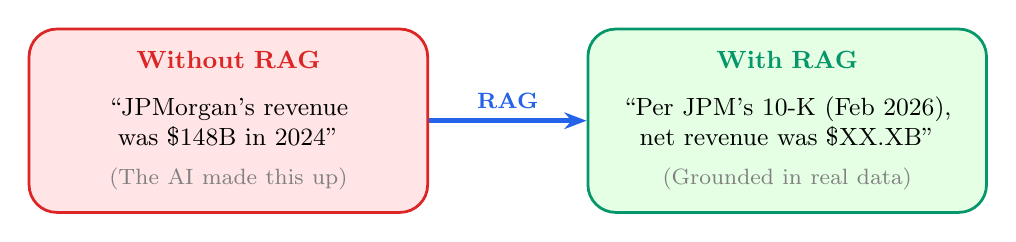
\begin{tikzpicture}[
      bubble/.style={rounded corners=10pt, minimum width=5cm, minimum height=2cm,
                     text width=4.5cm, align=center, font=\small, inner sep=8pt}
    ]
      \node[bubble, fill=red!10, draw=accent4, line width=1pt] (bad) {
        \textbf{\color{accent4}Without RAG}\\[6pt]
        ``JPMorgan's revenue was \$148B in 2024''\\[3pt]
        {\footnotesize\color{gray} (The AI made this up)}
      };

      \node[bubble, fill=green!10, draw=accent2, line width=1pt, right=2cm of bad] (good) {
        \textbf{\color{accent2}With RAG}\\[6pt]
        ``Per JPM's 10-K (Feb 2026), net revenue was \$XX.XB''\\[3pt]
        {\footnotesize\color{gray} (Grounded in real data)}
      };

      \draw[-{Stealth[length=8pt]}, line width=2pt, accent] (bad) -- (good)
        node[midway, above, font=\footnotesize\bfseries\color{accent}] {RAG};
    \end{tikzpicture}
  \end{center}

  \vspace{0.5cm}
  In banking, \textbf{accuracy is non-negotiable}. RAG ensures every AI answer
  is traceable to a source document.
\end{frame}

% ═══════════════════════════════════════════════════════════════════════════════
% 3. RAG
% ═══════════════════════════════════════════════════════════════════════════════
\section{RAG: Grounding AI in Facts}

\begin{frame}{What is RAG?}
  \textbf{Retrieval-Augmented Generation} = Search + AI

  \vspace{0.3cm}
  \begin{center}
    \begin{tikzpicture}[
      stp/.style={rounded corners=8pt, minimum width=3cm, minimum height=2cm,
                   text width=2.6cm, align=center, font=\small, inner sep=6pt},
      arr/.style={-{Stealth[length=8pt]}, line width=1.5pt, darkbg}
    ]
      \node[stp, fill=blue!12] (q) {
        \faUser\\[4pt]
        \textbf{Question}\\[2pt]
        {\footnotesize ``What risks does JPM face?''}
      };

      \node[stp, fill=amber!15, right=1.2cm of q] (search) {
        \faSearch\\[4pt]
        \textbf{Search}\\[2pt]
        {\footnotesize Find relevant paragraphs}
      };

      \node[stp, fill=green!12, right=1.2cm of search] (read) {
        \faFile\\[4pt]
        \textbf{Read}\\[2pt]
        {\footnotesize AI reads the top 5 results}
      };

      \node[stp, fill=purple!12, right=1.2cm of read] (ans) {
        \faRobot\\[4pt]
        \textbf{Answer}\\[2pt]
        {\footnotesize Cited, grounded response}
      };

      \draw[arr] (q) -- (search);
      \draw[arr] (search) -- (read);
      \draw[arr] (read) -- (ans);
    \end{tikzpicture}
  \end{center}

  \vspace{0.5cm}
  \begin{block}{The Analyst Analogy}
    RAG works like a junior analyst: \textbf{search} the filing cabinet,
    \textbf{read} the relevant pages, \textbf{write} a summary with citations.
  \end{block}
\end{frame}

\begin{frame}{How RAG Works Under the Hood}
  \begin{center}
    \begin{tikzpicture}[
      box/.style={rounded corners=6pt, minimum height=1.3cm, text width=3.2cm,
                  align=center, font=\small, inner sep=5pt},
      db/.style={rounded corners=6pt, draw=accent, fill=blue!8,
                 minimum width=2.5cm, minimum height=1.5cm, font=\small, align=center, inner sep=5pt},
      arr/.style={-{Stealth[length=7pt]}, line width=1.2pt}
    ]
      % Documents
      \node[box, fill=gray!10] (docs) at (0,2) {
        \faFile~\textbf{10-K Filings}\\
        {\footnotesize 100 companies\\ 5 years each}
      };

      % Chunking
      \node[box, fill=amber!15] (chunk) at (4,2) {
        \faCut~\textbf{Chunk}\\
        {\footnotesize Split into 500-word\\paragraphs}
      };

      % Vector DB
      \node[db] (vdb) at (8,2) {
        \textbf{Vector}\\
        \textbf{Database}
      };

      % Query path
      \node[box, fill=blue!10] (query) at (0,-0.5) {
        \faUser~\textbf{Question}
      };

      \node[box, fill=green!10] (retrieve) at (4,-0.5) {
        \faSearch~\textbf{Retrieve}\\
        {\footnotesize Top 5 matches}
      };

      \node[box, fill=purple!10] (llm) at (8,-0.5) {
        \faRobot~\textbf{LLM}\\
        {\footnotesize Synthesise answer}
      };

      \node[box, fill=accent2!10] (answer) at (12,-0.5) {
        \faCheckCircle~\textbf{Answer}\\
        {\footnotesize With citations}
      };

      \draw[arr, accent3] (docs) -- (chunk);
      \draw[arr, accent3] (chunk) -- (vdb);
      \draw[arr, accent] (query) -- (retrieve);
      \draw[arr, accent, dashed] (vdb) -- (retrieve) node[midway, right, font=\tiny] {similarity};
      \draw[arr, accent] (retrieve) -- (llm);
      \draw[arr, accent2] (llm) -- (answer);

      % Labels
      \node[above=0.2cm of docs, font=\footnotesize\color{gray}] {One-time setup};
      \node[below=0.2cm of query, font=\footnotesize\color{gray}] {Every question};
    \end{tikzpicture}
  \end{center}
\end{frame}

\begin{frame}{Embeddings: How Machines ``Understand'' Text}
  \begin{center}
    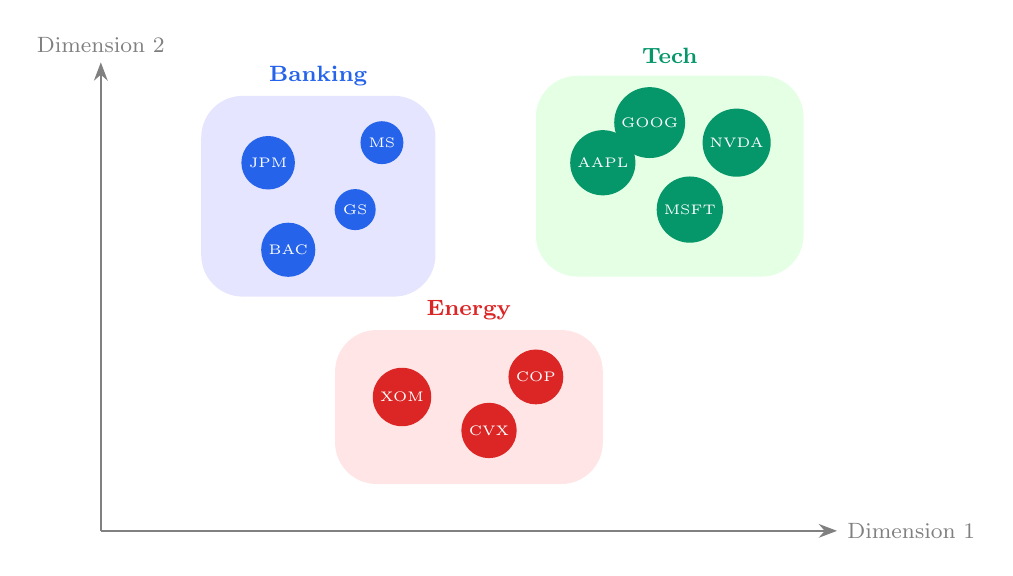
\begin{tikzpicture}[scale=0.85]
      % Axes
      \draw[-{Stealth}, gray, thick] (-1,-1) -- (10,-1) node[right, font=\footnotesize] {Dimension 1};
      \draw[-{Stealth}, gray, thick] (-1,-1) -- (-1,6) node[above, font=\footnotesize] {Dimension 2};

      % Banking cluster
      \fill[blue!10, rounded corners=15pt] (0.5,2.5) rectangle (4,5.5);
      \node[font=\footnotesize\color{accent}] at (2.25,5.8) {\textbf{Banking}};
      \node[circle, fill=accent, text=white, font=\tiny, inner sep=2pt] at (1.5,4.5) {JPM};
      \node[circle, fill=accent, text=white, font=\tiny, inner sep=2pt] at (2.8,3.8) {GS};
      \node[circle, fill=accent, text=white, font=\tiny, inner sep=2pt] at (1.8,3.2) {BAC};
      \node[circle, fill=accent, text=white, font=\tiny, inner sep=2pt] at (3.2,4.8) {MS};

      % Tech cluster
      \fill[green!10, rounded corners=15pt] (5.5,2.8) rectangle (9.5,5.8);
      \node[font=\footnotesize\color{accent2}] at (7.5,6.1) {\textbf{Tech}};
      \node[circle, fill=accent2, text=white, font=\tiny, inner sep=2pt] at (6.5,4.5) {AAPL};
      \node[circle, fill=accent2, text=white, font=\tiny, inner sep=2pt] at (7.8,3.8) {MSFT};
      \node[circle, fill=accent2, text=white, font=\tiny, inner sep=2pt] at (8.5,4.8) {NVDA};
      \node[circle, fill=accent2, text=white, font=\tiny, inner sep=2pt] at (7.2,5.1) {GOOG};

      % Energy cluster
      \fill[red!10, rounded corners=15pt] (2.5,-0.3) rectangle (6.5,2);
      \node[font=\footnotesize\color{accent4}] at (4.5,2.3) {\textbf{Energy}};
      \node[circle, fill=accent4, text=white, font=\tiny, inner sep=2pt] at (3.5,1.0) {XOM};
      \node[circle, fill=accent4, text=white, font=\tiny, inner sep=2pt] at (4.8,0.5) {CVX};
      \node[circle, fill=accent4, text=white, font=\tiny, inner sep=2pt] at (5.5,1.3) {COP};
    \end{tikzpicture}
  \end{center}

  \vspace{0.2cm}
  Companies that use \textbf{similar language} end up \textbf{close together} in vector space.\\
  \small A query about ``credit risk'' will land near the banking cluster --- not near energy or tech.
\end{frame}

% ═══════════════════════════════════════════════════════════════════════════════
% 4. AGENTS
% ═══════════════════════════════════════════════════════════════════════════════
\section{Agents: AI That Acts}

\begin{frame}{From Chatbot to Agent}
  \begin{center}
    \begin{tikzpicture}[
      box/.style={rounded corners=8pt, minimum width=5.5cm, minimum height=3cm,
                  text width=5cm, align=left, font=\small, inner sep=10pt}
    ]
      \node[box, fill=gray!10] (chat) {
        \textbf{\large\faComments~Chatbot}\\[6pt]
        \faAngleRight~Single question $\to$ single answer\\
        \faAngleRight~No memory between turns\\
        \faAngleRight~Cannot use tools\\
        \faAngleRight~Cannot plan
      };

      \node[box, fill=accent!8, right=1.5cm of chat] (agent) {
        \textbf{\large\color{accent}\faRobot~Agent}\\[6pt]
        \faAngleRight~Complex goal $\to$ multi-step plan\\
        \faAngleRight~Remembers what it found\\
        \faAngleRight~Uses tools (search, calculate)\\
        \faAngleRight~Reflects and adapts
      };

      \draw[-{Stealth[length=10pt]}, line width=2.5pt, accent]
        (chat.east) -- (agent.west);
    \end{tikzpicture}
  \end{center}
\end{frame}

\begin{frame}{The Agentic Loop}
  \begin{center}
    \begin{tikzpicture}[
      stp/.style={rounded corners=8pt, minimum width=2.5cm, minimum height=1.5cm,
                   align=center, font=\small\bfseries, inner sep=5pt},
      arr/.style={-{Stealth[length=7pt]}, line width=1.5pt, darkbg}
    ]
      \node[stp, fill=blue!15] (goal) at (0,0) {\faFlag\\Goal};
      \node[stp, fill=amber!20] (plan) at (3.5,0) {\faClipboardList\\Plan};
      \node[stp, fill=green!15] (act) at (7,0) {\faWrench\\Act};
      \node[stp, fill=purple!15] (observe) at (10.5,0) {\faEye\\Observe};
      \node[stp, fill=red!10] (reflect) at (7,-3) {\faBrain\\Reflect};
      \node[stp, fill=accent2!15] (answer) at (14,0) {\faCheckCircle\\Answer};

      \draw[arr] (goal) -- (plan);
      \draw[arr] (plan) -- (act);
      \draw[arr] (act) -- (observe);
      \draw[arr] (observe) -- (answer) node[midway, above, font=\tiny\color{gray}] {done?};

      % Loop back
      \draw[arr, accent4] (observe.south) -- ++(0,-0.8) -| (reflect.east);
      \draw[arr, accent4] (reflect.west) -| (plan.south);

      \node[font=\footnotesize\color{accent4}, below=0.1cm of reflect] {Need more info? Loop back.};
    \end{tikzpicture}
  \end{center}

  \vspace{0.3cm}
  \begin{exampleblock}{Example}
    \small
    \textbf{Goal:} ``Compare credit risk at JPM vs GS''\\
    \textbf{Plan:} Search JPM risks $\to$ Search GS risks $\to$ Compare $\to$ Synthesise\\
    \textbf{Reflect:} ``I found loan loss provisions but not derivatives exposure --- let me search again.''
  \end{exampleblock}
\end{frame}

\begin{frame}{Agent Tools = Analyst Toolkit}
  \begin{center}
    \begin{tikzpicture}[
      tool/.style={rounded corners=6pt, minimum width=4cm, minimum height=1.3cm,
                   text width=3.6cm, align=center, font=\small, inner sep=5pt},
      agent/.style={circle, fill=accent, text=white, minimum size=2cm,
                    font=\small\bfseries, align=center}
    ]
      \node[agent] (a) {\faRobot\\Agent};

      \node[tool, fill=blue!10, above right=1.5cm and 2cm of a] (search) {
        \faSearch~\textbf{Search}\\
        {\footnotesize Find relevant passages}
      };
      \node[tool, fill=green!10, right=2.5cm of a] (compare) {
        \faBalanceScale~\textbf{Compare}\\
        {\footnotesize Side-by-side analysis}
      };
      \node[tool, fill=amber!15, below right=1.5cm and 2cm of a] (risk) {
        \faExclamationTriangle~\textbf{Extract Risks}\\
        {\footnotesize Risk factor detection}
      };

      \draw[-{Stealth}, line width=1.2pt, accent] (a) -- (search);
      \draw[-{Stealth}, line width=1.2pt, accent2] (a) -- (compare);
      \draw[-{Stealth}, line width=1.2pt, accent3] (a) -- (risk);
    \end{tikzpicture}
  \end{center}

  \vspace{0.3cm}
  Like a Bloomberg terminal for an analyst --- the agent decides \textbf{which tool} to use
  and \textbf{when}, based on the question.
\end{frame}

% ═══════════════════════════════════════════════════════════════════════════════
% 5. LIVE DEMO
% ═══════════════════════════════════════════════════════════════════════════════
\section{Hands-On: Analysing 10-K Filings}

\begin{frame}{Our Dataset}
  \begin{center}
    \begin{tikzpicture}
      \node[rounded corners=10pt, fill=lightbg, text width=13cm, align=center,
            inner sep=15pt, font=\large] {
        \textbf{458 SEC 10-K Filings}\\[6pt]
        \normalsize
        100 S\&P 100 companies $\times$ up to 5 years\\[12pt]
        \begin{tikzpicture}
          \foreach \sector/\col/\x in {
            Tech/accent/0, Banking/accent3/2.5, Healthcare/accent2/5,
            Energy/accent4/7.5, Consumer/purple/10, Industrial/gray/12.5} {
            \node[rounded corners=4pt, fill=\col!15, minimum width=2cm,
                  minimum height=0.8cm, font=\footnotesize\bfseries] at (\x,0) {\sector};
          }
        \end{tikzpicture}
      };
    \end{tikzpicture}
  \end{center}

  \vspace{0.5cm}
  \begin{itemize}
    \item All filings publicly hosted on GitHub --- \textbf{no API keys needed}
    \item Accessible from Google Colab via HTTPS
    \item Real SEC data, not synthetic
  \end{itemize}
\end{frame}

\begin{frame}{The Pipeline We Built}
  \begin{center}
    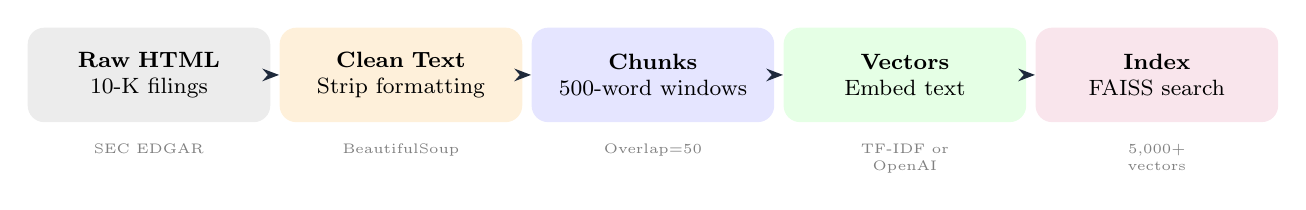
\begin{tikzpicture}[
      stp/.style={rounded corners=6pt, minimum height=1.2cm, text width=2.8cm,
                  align=center, font=\footnotesize, inner sep=4pt},
      arr/.style={-{Stealth[length=6pt]}, line width=1.2pt, darkbg},
      lbl/.style={font=\tiny\color{gray}, align=center}
    ]
      \node[stp, fill=gray!15] (raw) at (0,0) {\textbf{Raw HTML}\\10-K filings};
      \node[stp, fill=amber!15] (clean) at (3.2,0) {\textbf{Clean Text}\\Strip formatting};
      \node[stp, fill=blue!10] (chunk) at (6.4,0) {\textbf{Chunks}\\500-word windows};
      \node[stp, fill=green!10] (embed) at (9.6,0) {\textbf{Vectors}\\Embed text};
      \node[stp, fill=purple!10] (index) at (12.8,0) {\textbf{Index}\\FAISS search};

      \draw[arr] (raw) -- (clean);
      \draw[arr] (clean) -- (chunk);
      \draw[arr] (chunk) -- (embed);
      \draw[arr] (embed) -- (index);

      \node[lbl, below=0.15cm of raw] {SEC EDGAR};
      \node[lbl, below=0.15cm of clean] {BeautifulSoup};
      \node[lbl, below=0.15cm of chunk] {Overlap=50};
      \node[lbl, below=0.15cm of embed] {TF-IDF or\\OpenAI};
      \node[lbl, below=0.15cm of index] {5,000+\\vectors};
    \end{tikzpicture}
  \end{center}

  \vspace{0.8cm}
  \begin{center}
    {\Large\color{accent} $\Downarrow$}\\[0.3cm]
    \textbf{Let's switch to the live notebook.}
  \end{center}
\end{frame}

\begin{frame}[plain]
  \begin{center}
    \vspace{2cm}
    {\Huge\color{accent}\faLaptopCode}\\[1cm]
    {\LARGE\bfseries Live Demo}\\[0.5cm]
    {\large Part I: TF-IDF + Rule-Based Agent}\\[0.3cm]
    {\normalsize\color{gray} Sections 1--8 of the notebook}
  \end{center}
\end{frame}

% ═══════════════════════════════════════════════════════════════════════════════
% 6. FROM PROTOTYPE TO PRODUCTION
% ═══════════════════════════════════════════════════════════════════════════════
\section{From Prototype to Production}

\begin{frame}{The Upgrade Path}
  \begin{center}
    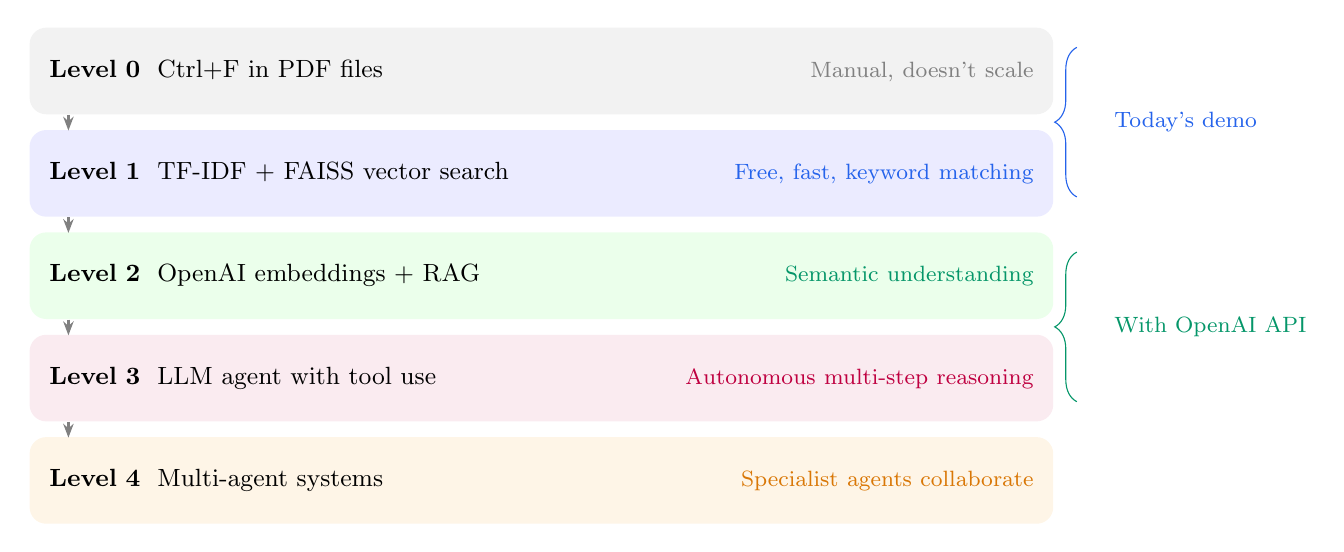
\begin{tikzpicture}[
      level/.style={rounded corners=6pt, minimum width=13cm, minimum height=1.1cm,
                    text width=12.5cm, align=left, font=\small, inner sep=6pt},
      arr/.style={-{Stealth[length=5pt]}, line width=1pt, gray}
    ]
      \node[level, fill=gray!10] (l0) at (0,4) {
        \textbf{Level 0}~~Ctrl+F in PDF files \hfill {\footnotesize\color{gray} Manual, doesn't scale}
      };
      \node[level, fill=blue!8] (l1) at (0,2.7) {
        \textbf{Level 1}~~TF-IDF + FAISS vector search \hfill {\footnotesize\color{accent} Free, fast, keyword matching}
      };
      \node[level, fill=green!8] (l2) at (0,1.4) {
        \textbf{Level 2}~~OpenAI embeddings + RAG \hfill {\footnotesize\color{accent2} Semantic understanding}
      };
      \node[level, fill=purple!8] (l3) at (0,0.1) {
        \textbf{Level 3}~~LLM agent with tool use \hfill {\footnotesize\color{purple} Autonomous multi-step reasoning}
      };
      \node[level, fill=amber!10] (l4) at (0,-1.2) {
        \textbf{Level 4}~~Multi-agent systems \hfill {\footnotesize\color{accent3} Specialist agents collaborate}
      };

      \draw[arr] (l0.south west) ++(0.5,0) -- ++(0,-0.2);
      \draw[arr] (l1.south west) ++(0.5,0) -- ++(0,-0.2);
      \draw[arr] (l2.south west) ++(0.5,0) -- ++(0,-0.2);
      \draw[arr] (l3.south west) ++(0.5,0) -- ++(0,-0.2);

      % Annotations
      \draw[decorate, decoration={brace, amplitude=8pt, mirror}, accent]
        (6.8, 4.3) -- (6.8, 2.4) node[midway, right=10pt, font=\footnotesize, text=accent] {Today's demo};
      \draw[decorate, decoration={brace, amplitude=8pt, mirror}, accent2]
        (6.8, 1.7) -- (6.8, -0.2) node[midway, right=10pt, font=\footnotesize, text=accent2] {With OpenAI API};
    \end{tikzpicture}
  \end{center}
\end{frame}

\begin{frame}{TF-IDF vs OpenAI Embeddings}
  \begin{center}
    \renewcommand{\arraystretch}{1.4}
    \begin{tabular}{l >{\raggedright\arraybackslash}p{4.5cm} >{\raggedright\arraybackslash}p{4.5cm}}
      \toprule
      & \textbf{TF-IDF} & \textbf{OpenAI Embeddings} \\
      \midrule
      \textbf{Approach} & Count words, weight by rarity & Neural network trained on billions of texts \\
      \textbf{Synonyms?} & ``revenue'' $\neq$ ``sales'' & ``revenue'' $\approx$ ``sales'' \\
      \textbf{Context?} & ``bank'' (river) = ``bank'' (finance) & Understands the difference \\
      \textbf{Cost} & Free & \$0.02 per 1M tokens \\
      \textbf{Best for} & Prototyping, keyword search & Production, semantic search \\
      \bottomrule
    \end{tabular}
  \end{center}

  \vspace{0.5cm}
  \small\color{gray}
  In financial text, this matters: ``provisions for credit losses'', ``allowance for loan losses'',
  and ``expected credit losses'' all mean the same thing. Only neural embeddings understand this.
\end{frame}

\begin{frame}[plain]
  \begin{center}
    \vspace{2cm}
    {\Huge\color{accent2}\faRocket}\\[1cm]
    {\LARGE\bfseries Live Demo}\\[0.5cm]
    {\large Part II: OpenAI Embeddings + LLM Agent}\\[0.3cm]
    {\normalsize\color{gray} Sections 10--13 of the notebook}
  \end{center}
\end{frame}

% ═══════════════════════════════════════════════════════════════════════════════
% 7. THE BANKING OPPORTUNITY
% ═══════════════════════════════════════════════════════════════════════════════
\section{The Banking Opportunity}

\begin{frame}{Use Cases Across the Bank}
  \begin{center}
    \begin{tikzpicture}[
      card/.style={rounded corners=6pt, minimum width=4.8cm, minimum height=2cm,
                   text width=4.4cm, align=left, font=\small, inner sep=8pt}
    ]
      \node[card, fill=blue!8] (risk) at (0,2.2) {
        \textbf{\color{accent}\faShield*~Risk Management}\\[3pt]
        {\footnotesize ``Flag all material litigation across 50 counterparty filings''}
      };
      \node[card, fill=green!8] (comp) at (5.5,2.2) {
        \textbf{\color{accent2}\faBalanceScale~Compliance}\\[3pt]
        {\footnotesize ``Do our portfolio companies disclose TCFD-aligned climate risks?''}
      };
      \node[card, fill=amber!10] (credit) at (0,-0.5) {
        \textbf{\color{accent3}\faUniversity~Credit Analysis}\\[3pt]
        {\footnotesize ``Compare debt covenants across 10 borrowers''}
      };
      \node[card, fill=purple!8] (ma) at (5.5,-0.5) {
        \textbf{\color{purple}\faHandshake~M\&A Due Diligence}\\[3pt]
        {\footnotesize ``Review target's risk factors, contracts, and contingent liabilities''}
      };
      \node[card, fill=red!6] (audit) at (2.75,-3.2) {
        \textbf{\color{accent4}\faClipboardCheck~Audit}\\[3pt]
        {\footnotesize ``Verify extracted figures match the original filing --- automatically''}
      };
    \end{tikzpicture}
  \end{center}
\end{frame}

\begin{frame}{Impact: Time Savings}
  \begin{center}
    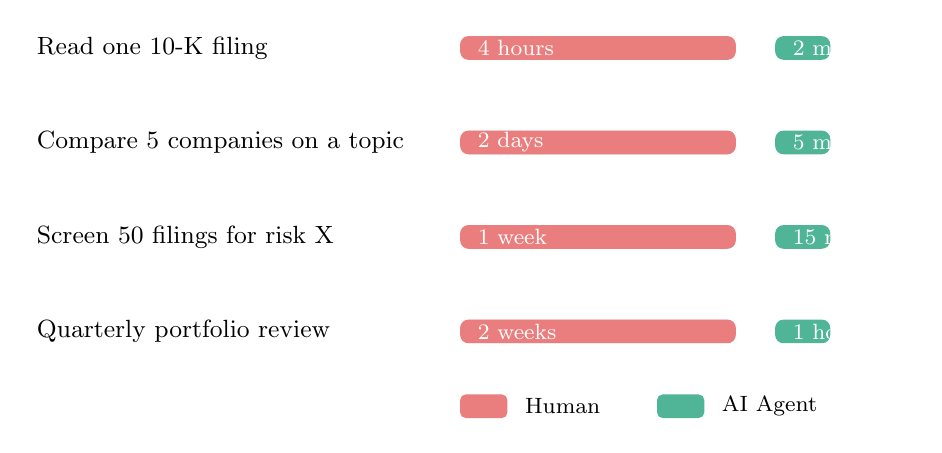
\begin{tikzpicture}
      \foreach \task/\human/\ai/\y in {
        {Read one 10-K filing}/4 hours/2 minutes/4,
        {Compare 5 companies on a topic}/2 days/5 minutes/2.8,
        {Screen 50 filings for risk X}/1 week/15 minutes/1.6,
        {Quarterly portfolio review}/2 weeks/1 hour/0.4} {
        \node[font=\small, anchor=west, text width=5cm] at (0,\y) {\task};
        \fill[gray!30, rounded corners=3pt] (5.5,\y-0.15) rectangle (9,\y+0.15);
        \fill[accent4!60, rounded corners=3pt] (5.5,\y-0.15) rectangle (9,\y+0.15);
        \node[font=\footnotesize, anchor=west, white] at (5.6,\y) {\human};
        \fill[accent2!70, rounded corners=3pt] (9.5,\y-0.15) rectangle (10.2,\y+0.15);
        \node[font=\footnotesize, anchor=west, white] at (9.6,\y) {\ai};
      }

      % Legend
      \fill[accent4!60, rounded corners=2pt] (5.5,-0.7) rectangle (6.1,-0.4);
      \node[font=\footnotesize, anchor=west] at (6.2,-0.55) {Human};
      \fill[accent2!70, rounded corners=2pt] (8,-0.7) rectangle (8.6,-0.4);
      \node[font=\footnotesize, anchor=west] at (8.7,-0.55) {AI Agent};
    \end{tikzpicture}
  \end{center}

  \vspace{0.3cm}
  \begin{alertblock}{Key insight}
    The value isn't replacing analysts --- it's \textbf{freeing them} for higher-order judgment.
  \end{alertblock}
\end{frame}

% ═══════════════════════════════════════════════════════════════════════════════
% 8. RISKS & GOVERNANCE
% ═══════════════════════════════════════════════════════════════════════════════
\section{Risks \& Governance}

\begin{frame}{What Can Go Wrong}
  \begin{columns}[T]
    \begin{column}{0.48\textwidth}
      \textbf{\color{accent4} Technical Risks}
      \begin{itemize}
        \item \textbf{Hallucination} --- AI states facts not in the source
        \item \textbf{Retrieval failure} --- wrong documents fetched
        \item \textbf{Stale data} --- filings not updated
        \item \textbf{Context limits} --- can't read entire filings at once
      \end{itemize}
    \end{column}
    \begin{column}{0.48\textwidth}
      \textbf{\color{accent3} Organisational Risks}
      \begin{itemize}
        \item \textbf{Over-reliance} --- trusting AI without verification
        \item \textbf{Data leakage} --- sensitive data sent to APIs
        \item \textbf{Regulatory} --- explainability requirements
        \item \textbf{Liability} --- who's responsible for AI errors?
      \end{itemize}
    \end{column}
  \end{columns}
\end{frame}

\begin{frame}{Governance Framework}
  \begin{center}
    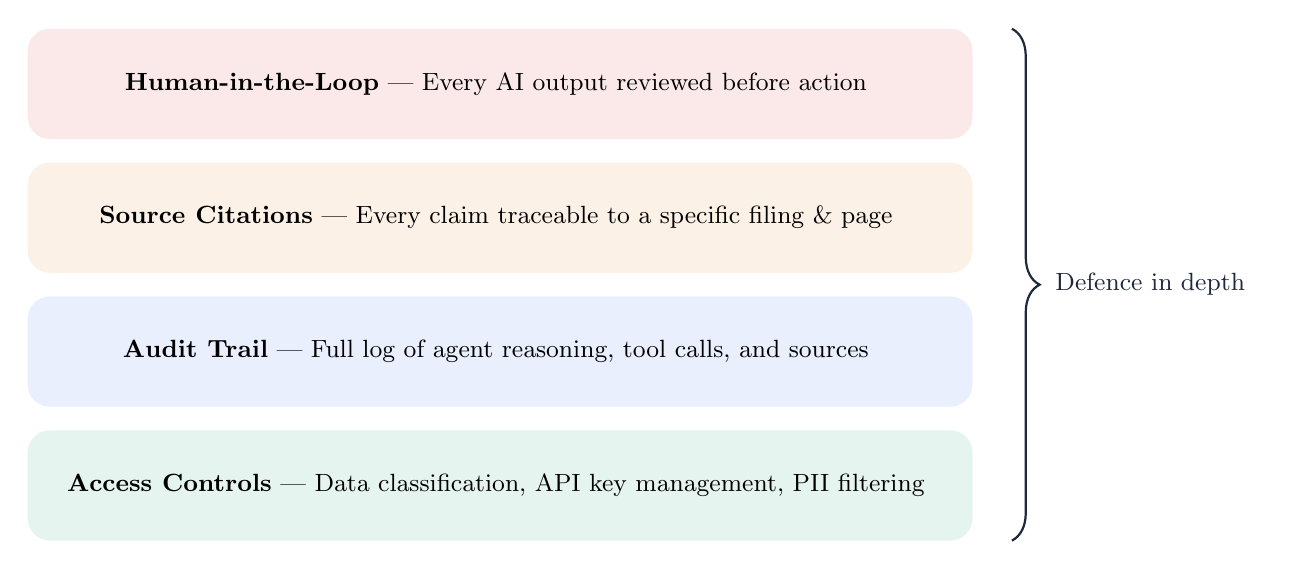
\begin{tikzpicture}[
      layer/.style={rounded corners=8pt, minimum width=12cm, minimum height=1.4cm,
                    align=center, font=\small, inner sep=6pt}
    ]
      \node[layer, fill=accent4!10] (l1) at (0,3.5) {
        \textbf{Human-in-the-Loop} --- Every AI output reviewed before action
      };
      \node[layer, fill=accent3!10] (l2) at (0,1.8) {
        \textbf{Source Citations} --- Every claim traceable to a specific filing \& page
      };
      \node[layer, fill=accent!10] (l3) at (0,0.1) {
        \textbf{Audit Trail} --- Full log of agent reasoning, tool calls, and sources
      };
      \node[layer, fill=accent2!10] (l4) at (0,-1.6) {
        \textbf{Access Controls} --- Data classification, API key management, PII filtering
      };

      \draw[decorate, decoration={brace, amplitude=10pt}, darkbg, thick]
        (6.5, 4.2) -- (6.5, -2.3)
        node[midway, right=12pt, font=\small, text width=2.5cm, align=left] {
          Defence in depth
        };
    \end{tikzpicture}
  \end{center}
\end{frame}

% ═══════════════════════════════════════════════════════════════════════════════
% CLOSING
% ═══════════════════════════════════════════════════════════════════════════════

\begin{frame}{Key Takeaways}
  \begin{enumerate}
    \setlength\itemsep{12pt}
    \item \textbf{RAG eliminates hallucination} by grounding every answer in real documents
    \item \textbf{Agents go beyond Q\&A} --- they plan, search, reflect, and iterate
    \item \textbf{The technology is ready today} --- OpenAI embeddings + GPT-4o + FAISS
    \item \textbf{Start small, scale fast} --- prototype in a notebook, deploy behind your firewall
    \item \textbf{Governance is essential} --- human oversight, citations, and audit trails
  \end{enumerate}
\end{frame}

\begin{frame}[plain]
  \begin{center}
    \vspace{1.5cm}
    {\Huge\bfseries Thank You}\\[1cm]
    {\Large Questions?}\\[1.5cm]

    \begin{tikzpicture}
      \node[rounded corners=8pt, fill=lightbg, inner sep=12pt, text width=10cm, align=center] {
        \faGithub~~\texttt{github.com/SMalamud/sec-10k-downloader}\\[6pt]
        \faLaptopCode~~Open in Colab: click the link in the README
      };
    \end{tikzpicture}
  \end{center}
\end{frame}

\end{document}
